\documentclass[letter,11pt]{article}

\usepackage[spanish,es-nodecimaldot]{babel}
\usepackage[utf8]{inputenc}

\usepackage{lmodern}
\usepackage[T1]{fontenc}
\usepackage{textcomp}

\usepackage{framed}
\usepackage[svgnames]{xcolor}
\colorlet{shadecolor}{Gainsboro!50}

\usepackage[shortlabels]{enumitem}
\usepackage{graphicx}
\usepackage{pstricks}
\usepackage{amsmath}

\usepackage{anysize}
\marginsize{3cm}{2cm}{2cm}{3cm}

\usepackage{fancyhdr}
\usepackage{lastpage}
\pagestyle{fancy}
\fancyhf{}
\fancyhead[LE,RO]{Física Básica II}
\fancyfoot[CO,CE]{\thepage\ de \pageref{LastPage}}

\special{papersize=215.9mm,279.4mm}

\usepackage[
    pdfauthor={Carlos Eduardo Caballero Burgoa},%
    pdftitle={Física Básica II},%
    pdfsubject={Tarea 23},%
    colorlinks,%
    citecolor=black,%
    filecolor=black,%
    linkcolor=black,%
    urlcolor=black,
    breaklinks]{hyperref}
\usepackage{breakurl}

\newcommand{\blankpage}{
\newpage
\thispagestyle{empty}
\mbox{}
\newpage
}

\renewcommand{\arraystretch}{1.2}

\begin{document}

\begin{center}
    {\Large \bf{Tarea \#23}}
\end{center}

Analice el sistema físico siguiente:
\\

\begin{figure}[!h]
\centering
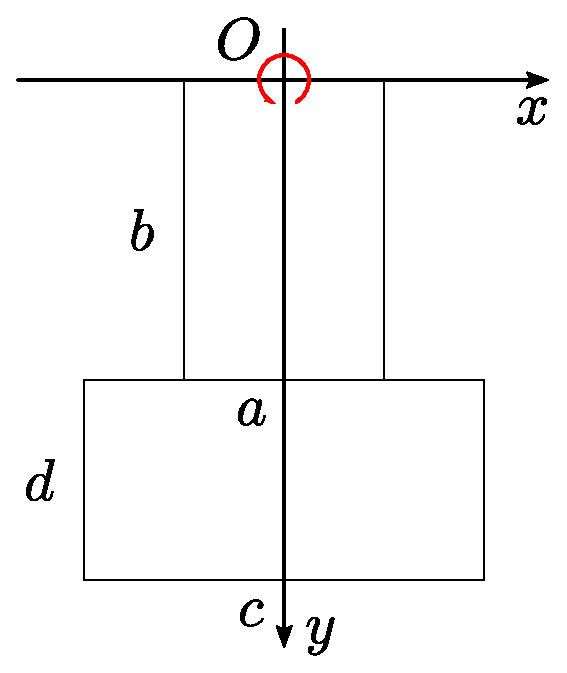
\includegraphics[scale=0.50]{resources/f1.eps}
\end{figure}
\vspace{0.2cm}

\textbf{Solución:} \\

\underline{Centro de masa:}

Centro de masa de la pieza $ab$:

\begin{equation*}
    \vec{r}_{ab} = (0, b/2)
\end{equation*}
\vspace{-0.1cm}

Centro de masa de la pieza $cd$:

\begin{equation*}
    \vec{r}_{cd} = (0, b + d/2)
\end{equation*}
\vspace{-0.1cm}

Centro de masa total:

\begin{equation}
    \vec{r}_{t} = \left(0, \frac{1}{2} \left(b/2 + b + d/2\right)\right) = \left(0, \frac{3b + d}{8}\right)
\end{equation}
\vspace{0.3cm}

\underline{Momento de inercia:}

Momento de inercia de la pieza $ab$:

\begin{equation*}
    I_{cm} = \frac{1}{12} M (a^2 + b^2)
\end{equation*}
\begin{equation*}
    I_{O1} = \frac{1}{12} M (a^2 + b^2) + M \left(\frac{b}{2}\right)^2 = \frac{1}{12} M (a^2 + 3b^2)
\end{equation*}
\vspace{-0.1cm}

Momento de inercia de la pieza $cd$:

\begin{equation*}
    I_{cm} = \frac{1}{12} M (c^2 + d^2)
\end{equation*}
\begin{equation*}
    I_{O2} = \frac{1}{12} M (a^2 + b^2) + M \left(b + \frac{d}{2}\right)^2 = \frac{1}{12} M (a^2 + 13 b^2 + bd + 3 d^2)
\end{equation*}
\vspace{-0.1cm}

Momento de inercia total:

\begin{equation*}
    I_{t} = I_{O1} + I_{O2} = \frac{1}{12} M (a^2 + 3b^2) +  \frac{1}{12} M (a^2 + 13 b^2 + bd + 3 d^2)
\end{equation*}
\begin{equation}
    I_{t} = \frac{1}{12} M (2a^2 + 16 b^2 + bd + 3d^2)
\end{equation}

\end{document}

